\documentclass[12pt,a4paper]{article}

\usepackage[margin=1in]{geometry}
\usepackage{setspace}
\usepackage{graphicx}
\usepackage{booktabs}
\usepackage{longtable}
\usepackage{hyperref}

\onehalfspacing
\hypersetup{colorlinks=true, linkcolor=blue, urlcolor=blue}

\title{Online Appendix:\\Predicting Inflation Contagion: A Spatio-Temporal Graph Neural Network Approach to Global Trade}
\author{Rayyan Asim \\ Independent Researcher \\ \texttt{mrayanasim09@gmail.com}}
\date{}

\begin{document}
\maketitle

\section{Hyperparameter Grid Search}
\label{sec:grid}

Table~\ref{tab:grid} reports validation RMSE for all 18 configurations searched in Milestone~7.
The selected model uses learning rate $5\times10^{-4}$, dropout 0.2, and two GCN layers (lowest validation RMSE 1.252).

\begin{longtable}{rrrr}
  \caption{Hyperparameter grid search on validation RMSE (2019Q1--2020Q4).}
  \label{tab:grid} \\
  \toprule
  Learning rate & Dropout & GCN layers & Val RMSE \\
  \midrule
  \endfirsthead
  \toprule
  Learning rate & Dropout & GCN layers & Val RMSE \\
  \midrule
  \endhead
    0.0005 & 0.2 & 2 & 1.252 \\
    0.0005 & 0.3 & 2 & 1.252 \\
    0.0005 & 0.4 & 2 & 1.252 \\
    0.0010 & 0.2 & 2 & 1.253 \\
    0.0010 & 0.3 & 2 & 1.253 \\
    0.0010 & 0.4 & 2 & 1.253 \\
    0.0005 & 0.2 & 1 & 1.254 \\
    0.0005 & 0.3 & 1 & 1.254 \\
    0.0005 & 0.4 & 1 & 1.254 \\
    0.0010 & 0.2 & 1 & 1.256 \\
    0.0010 & 0.3 & 1 & 1.256 \\
    0.0010 & 0.4 & 1 & 1.256 \\
    0.0030 & 0.2 & 1 & 1.257 \\
    0.0030 & 0.3 & 1 & 1.257 \\
    0.0030 & 0.4 & 1 & 1.257 \\
    0.0030 & 0.2 & 2 & 1.258 \\
    0.0030 & 0.3 & 2 & 1.258 \\
    0.0030 & 0.4 & 2 & 1.258 \\
  \bottomrule
\end{longtable}

\section{Supplementary Explainability Figures}

\subsection{Germany: Domestic vs.\ Trade Attribution (2020Q2)}

\begin{figure}[ht]
  \centering
  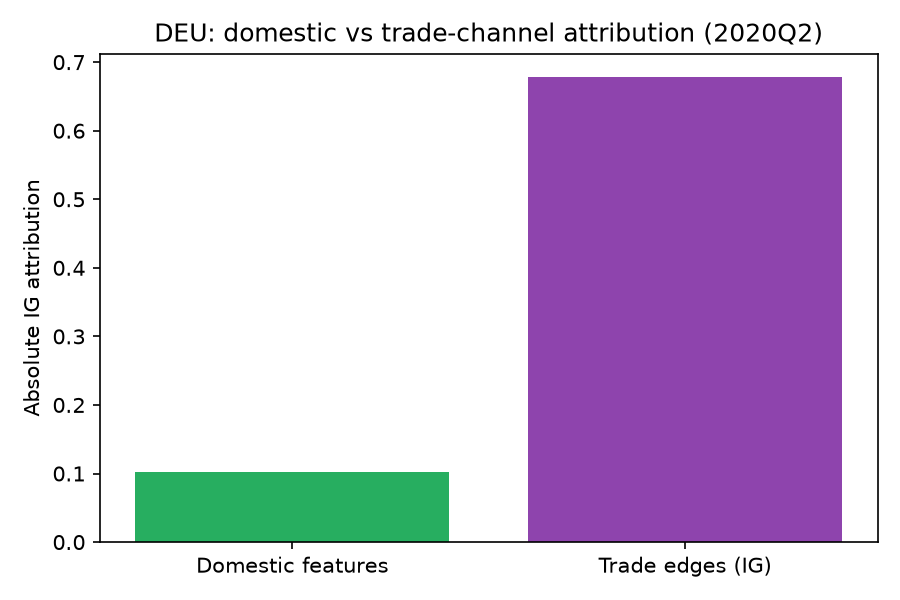
\includegraphics[width=0.75\linewidth]{figures/covid_supply_chain_domestic_vs_trade_DEU.png}
  \caption{Decomposition of Integrated Gradients attributions for Germany during the COVID supply-chain period (2020Q2).}
\end{figure}

\subsection{Germany: Domestic vs.\ Trade Attribution (2022Q2)}

\begin{figure}[ht]
  \centering
  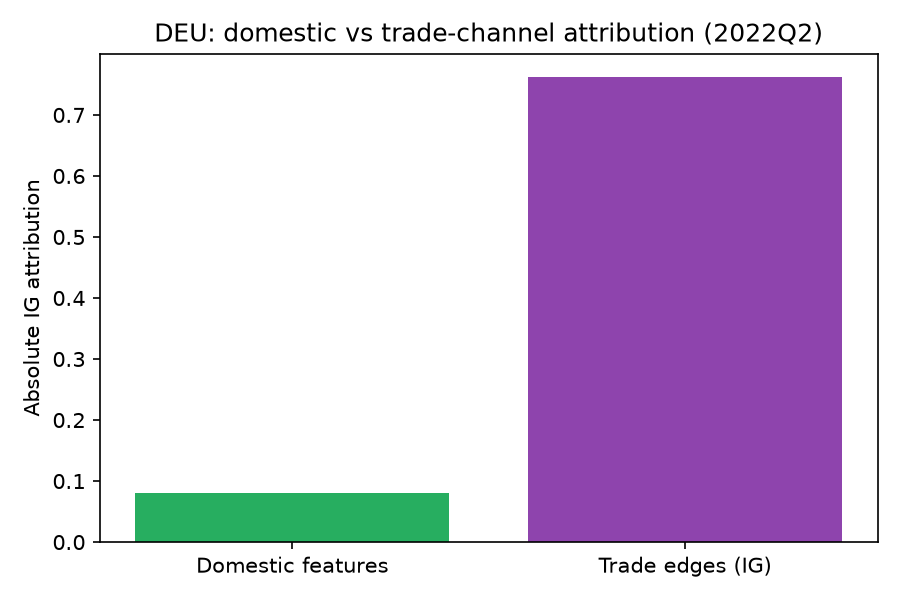
\includegraphics[width=0.75\linewidth]{figures/energy_shock_2022_domestic_vs_trade_DEU.png}
  \caption{Decomposition of Integrated Gradients attributions for Germany during the 2022 energy shock (2022Q2).}
\end{figure}

\subsection{Indonesia: Signed Partner Attributions (2022Q2)}

\begin{figure}[ht]
  \centering
  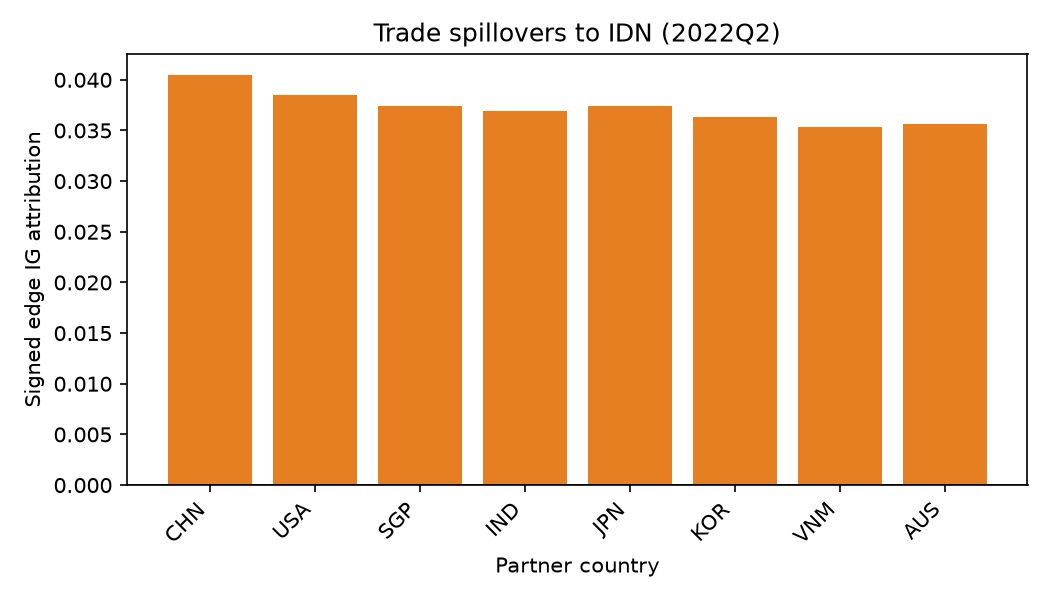
\includegraphics[width=0.75\linewidth]{figures/partner_spillover_heatmap.png}
  \caption{Signed edge attributions for Indonesia's top trade partners (2022Q2).}
\end{figure}

\subsection{Indonesia: Domestic vs.\ Trade Attribution (2022Q2)}

\begin{figure}[ht]
  \centering
  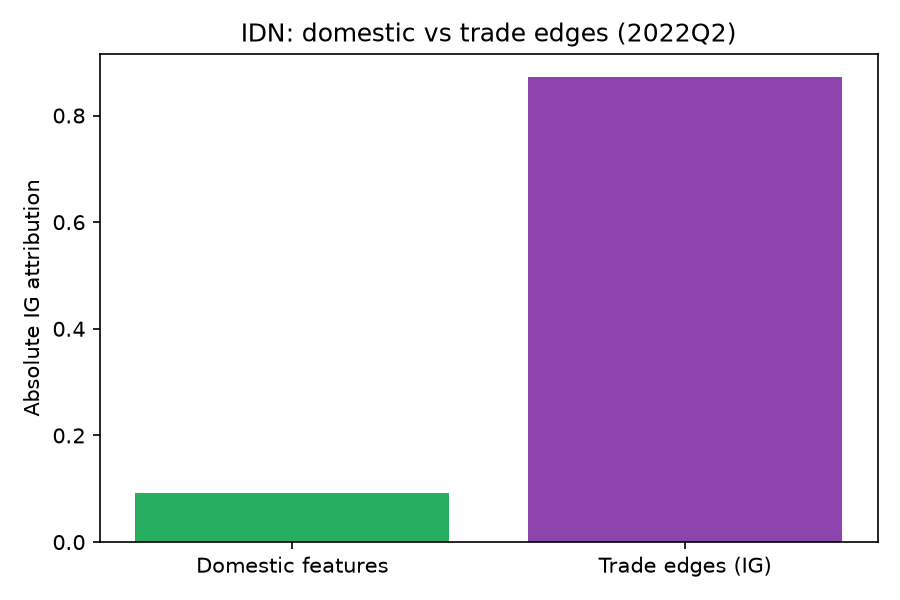
\includegraphics[width=0.75\linewidth]{figures/partner_spillover_domestic_vs_trade.png}
  \caption{Indonesia trade-versus-domestic attribution ratio (9.44), highest in the panel at 2022Q2.}
\end{figure}

\section{Country List}

Table~\ref{tab:countries} lists the 23 ISO3 codes in the estimation panel.

\begin{table}[ht]
  \centering
  \caption{Estimation panel (23 countries).}
  \label{tab:countries}
  \begin{tabular}{llllll}
    \toprule
    ARG & AUS & BRA & CAN & CHE & CHN \\
    DEU & FRA & GBR & IDN & IND & ITA \\
    JPN & KOR & MEX & NLD & RUS & SAU \\
    SGP & TUR & USA & VNM & ZAF & \\
    \bottomrule
  \end{tabular}
\end{table}

\section{Replication Instructions}

Full replication code is provided in \texttt{Replication\_Code.zip}.
Macro data download automatically via \texttt{python -m src.download\_macro}.
CEPII BACI bulk files must be obtained separately from CEPII (several GB; not included in the zip).
See \texttt{REPLICATION\_README.md} inside the zip for the complete pipeline from raw data through explainability figures.

\end{document}
